%\section{Electrical aspects}

\section{Electronics and Communication}
Our electronics were designed to handle all low-level tasks that are
required to move AquaTux, acquire sensor data and trigger
electrical systems like the  marker droppers. The main goal
of the electronics is to allow the AUV to be driven with only
high-level heading and depth commands. The electronics are responsible for
executing the commands and controlling their results (e.g. depth or
heading) in a ``black box'' fashion. This level of separation, created by our command
communication protocol, provides the option of tethered communication directly to the Navigation board via RS232 or through the computer's ethernet port
that relays commands to the Navigation board.

\subsection{Navigation Board}
The Navigation Board provides signal conditioning and circuitry interfacing for all sensors, including the Motor Boards and Peripheral Control Boards. In addition, all communication either goes to or through the navigation board. This is also
the access point when the computer has to communicate with the lower level
electronics. It features an LPC2129 microcontroller (MCU) at its core, operating at
12Mhz and utilizes Control Area Network (CAN), two-wire serial I2C,
and RS232 protocols to communicate with the Motor Boards, Peripheral
Control Board / Batteries, and the Computer respectively. The
navigation board reads the heading from an HMR3300 Digital Compass
connected through a serial port.  An analog pressure sensor, MPX4115, provides a linear
voltage representation of the depth, and is also connected to the
navigation board feeding directly into a successive approximation A/D
in the LPC2129. This board is the key element in handling all low-level operations such as movement and data collection.

\subsection{Peripheral Control Board}


The circuit board operates as an extension to the navigation board by
performing the tasks of actuating the marker droppers and debouncing
the custom-made leak sensors. The Peripheral Control Board uses
SN754410 quadruple half H-Bridge drivers: two of which are used to
actuate the marker droppers and one to fire the torpedo. The
Peripheral Control Board uses an ATmega48p MCU to control the half
H-bridge drivers, and query the leak sensors and the feedback switches
from the marker dropper. The microcontroller communicates with the
navigation board through the I2C network of the AUV.

\subsection{Motor Board}

The motor drivers are used to control the Seabotix BTD150 Thrusters
used on AquaTux.  There are a total of five motor drivers, one for
each thruster used on the AUV (Figure~\ref{mstack}). The motor drivers are based around the NXP
LPC2129 MCU which has number of features ideally suited to our
application, including a 4 channel SAR ADC, a 6-channel dual edge
triggered PWM module, a CAN module and a simple serial boot-loader.
The thrusters are controlled via current control, and other safety
features such as current limiting, and acceleration control are
implemented.  By receiving commands through the CAN bus, these Motor
Boards will ensure that the thrusters are never harmed by excessive
current during operation.

\begin{figure}
\begin{center}
 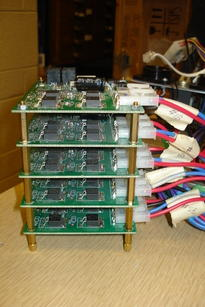
\includegraphics[width=1.5in]{fig/dsc06472} %1.34
\vspace{.05in}
\hrule
\caption{Stack of motor control boards on a CAN bus.}\label{mstack}
\end{center}
\end{figure}


The motor controller hardware is centered around a pair of Linear
Technology LT1160 half-bridge drivers which include high side charge
pumps, shoot through protection and undervoltage lockout. A number of
additional components were added to increase the bridge robustness
including TVS diodes, anti-parallel gate diodes and large on-board
bulk capacitors. Two types of sensors were integrated into the motor
board in order to sense motor function. Back EMF measurement
capability as well as motor current circuits were added. An active-RC
filter similar to that on the navigation board was used coupled with a
high side sense resistor and INA168 to measure the motor current.
Motor current measurement is critical as it must be kept below 4A to
prevent motor damage.

\section{Power Distribution}
AquaTux is powered by three 24V NiMH battery packs.  The three battery
packs each power a different section of the AUV.  Two packs directly
feed into the Motor Boards: one pack is used to power the three
vertical thrusters, and a second pack provides power for the two
horizontal thrusters.  The last battery pack provides power for the
rest of AquaTux after being conditioned by Switch Mode Power Supplies
(SMPS) to create two separate bus voltages. A 5V SMPS feeds the
Kontron SpeedMopsLcdPM PC104+ computer, while a 12V SMPS provides power to
all other modules of the AUV, which includes the navigation board,
cameras, and all other sensors. If other voltages are required for the
electronics, linear regulators are used to produce them.  In case of
emergency, relays toggled by magnetic switches are used to disconnect
the batteries from the rest of the AUV. Circuit breakers are also put
inline with the battery to act as both the fuse, and the power
switches for the AUV. The power architecture was designed to keep
board to board wiring simple by minimizing the number of bus voltages.

\subsection{Power Source}
The NiMH battery packs were custom designed by our team: each pack is
composed of 20 SY136T Sanyo nickel metal hydride batteries.  All
batteries are connected in series to form a 24V nominal battery pack
with a capacity of 4100mAh.  Each pack has its own protection
circuitry that utilizes an Atmega48p AVR as its MCU.  A gas gauging IC, BQ2013,
from Texas Instruments is used to track the charge status of the
battery. %BQ2013
For safety, the pack has a disconnect FET on the high side of the
battery.  This FET will disconnect the pack when the pack is drained
or at a temperature greater than 80 degrees Celsius. All battery packs
are connected to the I2C bus on the navigation board, allowing for
remote monitoring of the batteries at all time.

\subsection{Battery Charger}
The battery charger was also designed by our team and has at its core
an Atmega168p MCU.  This MCU monitors the voltage and
temperature of the battery pack being charged, and will automatically
terminate charging based on the temperature rise of the NiMH cells.
The charger must also communicate with the pack via I2C in order to
read the battery pack ID, and to ensure that the disconnect FET is
enabled for charging.  Charge current is set by utilizing a sense
resistor, and an opamp to control the gate voltage of a MOSFET.  The
MOSFET operates in saturation in order for us to appropriately limit
the charge current of the batteries. Because the voltage range of the
NiMH cells extends from 1.4V to 1.6V, the voltage supply required to
charge a 20 cell pack must be greater than 32V: we chose a 36V supply for cost-effectiveness.
